\documentclass[nofootinbib,tightenlines,nobibnotes,aps,prl,preprint,superscriptaddress]{revtex4-1}
\usepackage[utf8]{inputenc}	% Required for inputting international characters
\usepackage[T1]{fontenc} 		% Output font encoding for international characters
\usepackage{lmodern}				% nicer font
\usepackage{microtype}			% improv. of white-space

\usepackage{graphicx}				% Including figure files
\usepackage{amsmath}				% Advanced maths commands
\usepackage{amssymb}				% Extra maths symbols
\usepackage{siunitx}				% proper SI notation
\usepackage{csquotes}				% quotations and quotation marks
\usepackage{hyperref}				% referencing
\usepackage{cleveref}				% smart referencing (requires hyperref)
\usepackage{acro}						% abbreviations and nomenclature
\usepackage{tabu}						% advanced tabular enviroment
\usepackage{booktabs}				% simple table design scheme
\usepackage{threeparttable}	% for table notes
%\usepackage{caption}				
\usepackage{url}						% for pretty urls
\usepackage[all]{nowidow}		% tries to avoid widows
\usepackage[draft]{changes}	% track changes (manually)

\usepackage{ulem}

\usepackage{aas_macros}
% sets
\def \L {\mathbb{L}}
\def \N {\mathbb{N}}										% natural numbers
\def \Z {\mathbb{Z}}										% integral numbers
\def \Q {\mathbb{Q}}										% rational numbers
\def \R {\mathbb{R}}										% real numbers
\def \C {\mathbb{C}}										% complex numbers
\def \SO #1{\text{SO(#1)}}							% SO(n) group, orthonormal matrices
\def \so #1{\mathfrak{so}\text{(#1)}}		% so(n) algebra, anti-symmetric matrices


% important signs
\def \E			#1{\cdot 10^{#1}}					% scientific notation
\def \e			{\mathrm{e}}							% euler number
\def \d			{\mathop{}\!\mathrm{d}}							% differential
\def \i			{\mathfrak{i}}						% imaginary unit
\def \const {\mathrm{const}}					% constant expression
\def \other	{\mathrm{else}}						% else expression
\def \um		{\text{-}}								% small minus sign (useful for exponential or index notation)
\def \tp		{\text{t}}								% transpose sign for matrices (use as superscript)
\def \eye		{\mathbbm{1}}
\def \levicivita {\varepsilon}
\DeclareRobustCommand{\orderof}{\ensuremath{\mathcal{O}}}


% fraction
\newcommand\FRAC[2]{\frac{\displaystyle #1}{\displaystyle #2}} % large frac

% functions/operators
\def \tr		#1{\operatorname{tr}\bracket{#1}}
\def \var		{\mathrm{\delta}}
\DeclareMathOperator{\sgn}{sgn}
\DeclareMathOperator{\diag}{diag}
\DeclareMathOperator{\sinc}{sinc}
\DeclareMathOperator{\erf}{erf}
\DeclareMathOperator{\erfc}{erfc}
\DeclareMathOperator{\polylog}{Li}

\newcommand*\pFq[2]{{}_{#1}F_{#2}} % hyper geometric function


% brackets
\def \listset		#1{\left\{#1\right\}}									% {...}
\def \bracket		#1{\left(#1\right)}										% (...)
\def \sbracket	#1{\left\langle#1\right\rangle}				% <...>
%\def \qbracket	#1{\left[#1\right]}									% [...]
\def \braces		#1{\left\{#1\right\}}									% {...}
\def \abs				#1{\left|#1\right|}										% |...|

% brackets (v2)
\newcommand \qbracket[2][]{\left[\vphantom{#1}#2\right]}								% [...]

\def \integral	#1#2#3{\left[#1\right]^{#3}_{#2}}			% [...]_.^.
\def \at				#1#2{\left.{#1}\right|_{#2}}					% |_.

\def \bra				#1{\left<#1\right|}										% <...|
\def \ket				#1{\left|#1\right>}										% |...>
\def \braket		#1#2{\left<#1\right|\left.#2\right>}	% <...|...>

% operations [derivative]
\def \diff				#1#2{\frac{\d#1}{\d#2}}
\def \ddiff				#1#2{\frac{\d^2#1}{\d#2^2}}
\def \ndiff				#1#2#3{\frac{\d^{#3}#1}{\d#2^{#3}}}

\def \diffat			#1#2#3{\at{\diff{#1}{#2}}{#3}}
\def \ddiffat			#1#2#3{\at{\ddiff{#1}{#2}}{#3}}
\def \ndiffat			#1#2#3#4{\at{\ndiff{#1}{#2}{#3}}{#4}}

\def \diffpart		#1#2{\frac{\partial #1}{\partial #2}}
\def \ddiffpart		#1#2{\frac{\partial^2 #1}{\partial #2^2}}
\def \ndiffpart		#1#2#3{\frac{\partial^{#3}#1}{\partial#2^{#3}}}

\def \diffpartat	#1#2#3{\at{\diffpart{#1}{#2}}{#3}}
\def \ddiffpartat	#1#2#3{\at{\ddiffpart{#1}{#2}}{#3}}
\def \ndiffpartat	#1#2#3#4{\at{\ndiffpart{#1}{#2}{#3}}{#4}}

\def \todiffpart	#1#2{\frac{\partial #1}{\partial #2}\d#2}

% range/interval
\def \rangesim 		#1#2#3#4{#1 \sim #2\text{ -- }#3\,{#4}}

% data
\newcommand \val[2]{{#1}\,{#2}}	

% textual diferentials
\def \tdiff				#1#2{\d#1/\d#2}
\def \tddiff			#1#2{\d^2#1/\d#2^2}

% load figure
\def \loadfigure 	#1{\def\ROOTPATH{#1}\begin{figure}%
	\centering%
	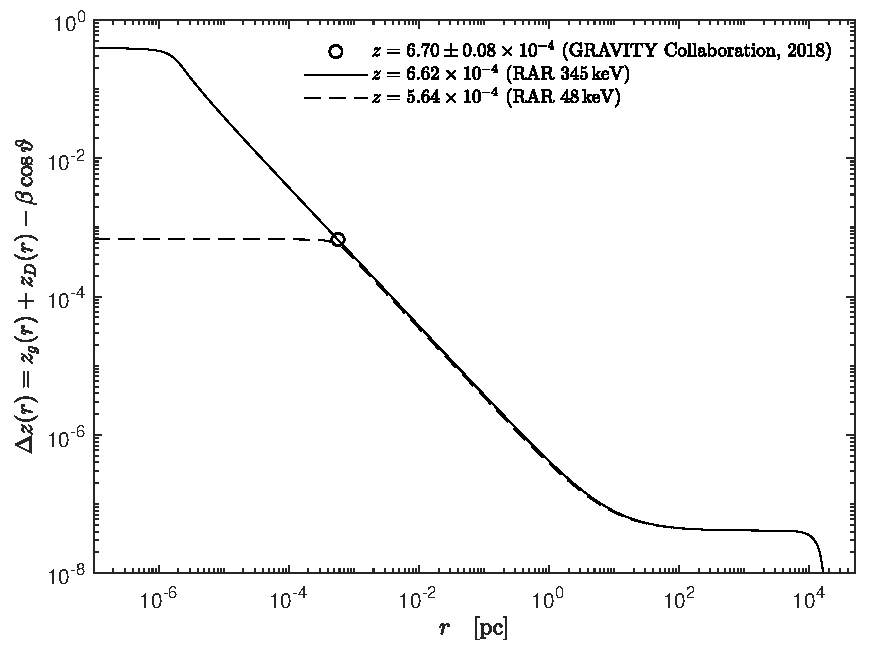
\includegraphics[width=\hsize]{\ROOTPATH/fig.pdf}
	\caption{Comparison of the inferred redshift correction at the S2 pericenter (circle) and the predicted curves of the RAR solutions as obtained in \citet{arguelles_novel_2018}.}%
	\label{fig:redshift}%
\end{figure}}

\hypersetup{
	colorlinks,
	linkcolor={red!50!black},
	citecolor={magenta},
	urlcolor={blue!80!black}
}

% change vector style to bold letter
\renewcommand{\vec}[1]{\mbox{\boldmath$#1$}}

% make tables less compact
\renewcommand{\arraystretch}{1.3}

% allow figures more space to cover before forcing into a seperate page
\renewcommand{\floatpagefraction}{.8}

% for continued figures
%\DeclareCaptionFormat{cont}{#1 (cont.)#2#3\par}

% define units
\DeclareSIUnit \c 			{\ensuremath{\mathit{c}}}
\DeclareSIUnit \parsec 	{pc}
\DeclareSIUnit \eV 			{eV}
\DeclareSIUnit \eVcc		{eV\per\c\squared}
\DeclareSIUnit \Msun 		{M_\odot}

% define authors
% nice colors are: orange, purple, olive, brown, cyan, magenata red, 
% not recommended are: black, white, gray, darkgray, blue, lime, yellow, pink
\definechangesauthor[name={Andreas}, color=orange]{ak}
\definechangesauthor[name={Carlos}, color=purple]{ca}
\definechangesauthor[name={Jorge}, color=olive]{jr}

% uncomment for hiding the author markup
%\setauthormarkup{}

% bibliography
%\bibliographystyle{elsarticle-num-names}

% change SI range
\sisetup{
	range-phrase	= \text{ -- },
	range-units		= single
}
%
%  These Macros are taken from the AAS TeX macro package version 5.2
%  and are compatible with the macros in the A&A document class
%  version 7.0
%  Include this file in your LaTeX source only if you are not using
%  the AAS TeX macro package or the A&A document class and need to
%  resolve the macro definitions in the TeX/BibTeX entries returned by
%  the ADS abstract service.
%
%  If you plan not to use this file to resolve the journal macros
%  rather than the whole AAS TeX macro package, you should save the
%  file as ``aas_macros.sty'' and then include it in your LaTeX paper
%  by using a construct such as:
%	\documentstyle[11pt,aas_macros]{article}
%
%  For more information on the AASTeX and A&A packages, please see:
%	http://aastex.aas.org
%       ftp://ftp.edpsciences.org/pub/aa/readme.html
%  For more information about ADS abstract server, please see:
%	http://adsabs.harvard.edu/ads_abstracts.html
%

% Abbreviations for journals.  The object here is to provide authors
% with convenient shorthands for the most "popular" (often-cited)
% journals; the author can use these markup tags without being concerned
% about the exact form of the journal abbreviation, or its formatting.
% It is up to the keeper of the macros to make sure the macros expand
% to the proper text.  If macro package writers agree to all use the
% same TeX command name, authors only have to remember one thing, and
% the style file will take care of editorial preferences.  This also
% applies when a single journal decides to revamp its abbreviating
% scheme, as happened with the ApJ (Abt 1991).

\let\jnlATstyle=\textrm
\def\refATjnl#1{{\jnlATstyle#1}}

\def\aj{\refATjnl{AJ}}                   % Astronomical Journal
\def\actaa{\refATjnl{Acta Astron.}}      % Acta Astronomica
\def\araa{\refATjnl{ARA\&A}}             % Annual Review of Astron and Astrophys
\def\apj{\refATjnl{ApJ}}                 % Astrophysical Journal
\def\apjl{\refATjnl{ApJ}}                % Astrophysical Journal, Letters
\def\apjs{\refATjnl{ApJS}}               % Astrophysical Journal, Supplement
\def\ao{\refATjnl{Appl.~Opt.}}           % Applied Optics
\def\apss{\refATjnl{Ap\&SS}}             % Astrophysics and Space Science
\def\aap{\refATjnl{A\&A}}                % Astronomy and Astrophysics
\def\aapr{\refATjnl{A\&A Rev.}}          % Astronomy and Astrophysics Reviews
\def\aaps{\refATjnl{A\&AS}}              % Astronomy and Astrophysics, Supplement
\def\azh{\refATjnl{AZh}}                 % Astronomicheskii Zhurnal
\def\baas{\refATjnl{BAAS}}               % Bulletin of the AAS
\def\bac{\refATjnl{Bull. astr. Inst. Czechosl.}}
                % Bulletin of the Astronomical Institutes of Czechoslovakia 
\def\caa{\refATjnl{Chinese Astron. Astrophys.}}
                % Chinese Astronomy and Astrophysics
\def\cjaa{\refATjnl{Chinese J. Astron. Astrophys.}}
                % Chinese Journal of Astronomy and Astrophysics
\def\icarus{\refATjnl{Icarus}}           % Icarus
\def\jcap{\refATjnl{J. Cosmology Astropart. Phys.}}
                % Journal of Cosmology and Astroparticle Physics
\def\jrasc{\refATjnl{JRASC}}             % Journal of the RAS of Canada
\def\memras{\refATjnl{MmRAS}}            % Memoirs of the RAS
\def\mnras{\refATjnl{MNRAS}}             % Monthly Notices of the RAS
\def\na{\refATjnl{New A}}                % New Astronomy
\def\nar{\refATjnl{New A Rev.}}          % New Astronomy Review
\def\pra{\refATjnl{Phys. Rev. A}}        % Physical Review A: General Physics
\def\prb{\refATjnl{Phys. Rev. B}}        % Physical Review B: Solid State
\def\prc{\refATjnl{Phys. Rev. C}}        % Physical Review C
\def\prd{\refATjnl{Phys. Rev. D}}        % Physical Review D
\def\pre{\refATjnl{Phys. Rev. E}}        % Physical Review E
\def\prl{\refATjnl{Phys. Rev. Lett.}}    % Physical Review Letters
\def\pasa{\refATjnl{PASA}}               % Publications of the Astron. Soc. of Australia
\def\pasp{\refATjnl{PASP}}               % Publications of the ASP
\def\pasj{\refATjnl{PASJ}}               % Publications of the ASJ
\def\rmxaa{\refATjnl{Rev. Mexicana Astron. Astrofis.}}%
                % Revista Mexicana de Astronomia y Astrofisica
\def\qjras{\refATjnl{QJRAS}}             % Quarterly Journal of the RAS
\def\skytel{\refATjnl{S\&T}}             % Sky and Telescope
\def\solphys{\refATjnl{Sol. Phys.}}      % Solar Physics
\def\sovast{\refATjnl{Soviet Ast.}}      % Soviet Astronomy
\def\ssr{\refATjnl{Space Sci. Rev.}}     % Space Science Reviews
\def\zap{\refATjnl{ZAp}}                 % Zeitschrift fuer Astrophysik
\def\nat{\refATjnl{Nature}}              % Nature
\def\iaucirc{\refATjnl{IAU Circ.}}       % IAU Cirulars
\def\aplett{\refATjnl{Astrophys. Lett.}} % Astrophysics Letters
\def\apspr{\refATjnl{Astrophys. Space Phys. Res.}}
                % Astrophysics Space Physics Research
\def\bain{\refATjnl{Bull. Astron. Inst. Netherlands}} 
                % Bulletin Astronomical Institute of the Netherlands
\def\fcp{\refATjnl{Fund. Cosmic Phys.}}  % Fundamental Cosmic Physics
\def\gca{\refATjnl{Geochim. Cosmochim. Acta}}   % Geochimica Cosmochimica Acta
\def\grl{\refATjnl{Geophys. Res. Lett.}} % Geophysics Research Letters
\def\jcp{\refATjnl{J. Chem. Phys.}}      % Journal of Chemical Physics
\def\jgr{\refATjnl{J. Geophys. Res.}}    % Journal of Geophysics Research
\def\jqsrt{\refATjnl{J. Quant. Spec. Radiat. Transf.}}
                % Journal of Quantitiative Spectroscopy and Radiative Transfer
\def\memsai{\refATjnl{Mem. Soc. Astron. Italiana}}
                % Mem. Societa Astronomica Italiana
\def\nphysa{\refATjnl{Nucl. Phys. A}}   % Nuclear Physics A
\def\physrep{\refATjnl{Phys. Rep.}}   % Physics Reports
\def\physscr{\refATjnl{Phys. Scr}}   % Physica Scripta
\def\planss{\refATjnl{Planet. Space Sci.}}   % Planetary Space Science
\def\procspie{\refATjnl{Proc. SPIE}}   % Proceedings of the SPIE

\let\astap=\aap
\let\apjlett=\apjl
\let\apjsupp=\apjs
\let\applopt=\ao



\begin{document}
\title{Preliminary results of the S2 redshift analysis within the RAR model}

% repeat the \author .. \affiliation  etc. as needed
% \email, \thanks, \homepage, \altaffiliation all apply to the current
% author. Explanatory text should go in the []'s, actual e-mail
% address or url should go in the {}'s for \email and \homepage.
% Please use the appropriate macro foreach each type of information
\author{C.~R.~Argüelles}
\email{carlos.arguelles@icranet.org}
\affiliation{\footnotesize Instituto de Astrofísica de La Plata (CCT La Plata, CONICET, UNLP), Paseo del Bosque, B1900FWA La Plata, Argentina}
\affiliation{\footnotesize ICRANet, Piazza della Repubblica 10, I--65122 Pescara, Italy}

\author{A. Krut}
\email{andreas.krut@icranet.org}
\affiliation{\footnotesize ICRANet, Piazza della Repubblica 10, I--65122 Pescara, Italy}

\author{J.~A.~Rueda}
\email{jorge.rueda@icra.it}
\affiliation{\footnotesize ICRANet, Piazza della Repubblica 10, I--65122 Pescara, Italy}
\affiliation{\footnotesize Dipartimento di Fisica and ICRA, Sapienza Università di Roma, P.le Aldo Moro 5, I--00185 Rome, Italy}
\affiliation{\footnotesize ICRANet-Rio, CBPF, Rua Dr.~Xavier Sigaud 150, Rio de Janeiro, RJ, 22290--180, Brazil}

\author{R.~Ruffini}
\email{ruffini@icra.it}
\affiliation{\footnotesize ICRANet, Piazza della Repubblica 10, I--65122 Pescara, Italy}
\affiliation{\footnotesize Dipartimento di Fisica and ICRA, Sapienza Università di Roma, P.le Aldo Moro 5, I--00185 Rome, Italy}
\affiliation{\footnotesize ICRANet-Rio, CBPF, Rua Dr.~Xavier Sigaud 150, Rio de Janeiro, RJ, 22290--180, Brazil}

\date{\today}


\begin{abstract}
The recent fly by of the S2 star through its pericenter allowed to verify relativistic effects in the galactic center based on the robust detection of the combined gravitational redshift and relativistic transverse Doppler effect for S2 \citep{2018A&A...615L..15G}. The detection of relativistic corrections for the S2 orbit are yet out of precision due to the large distance ($1400r_{\rm Sch}$) of the pericenter to an assumend BH in the galactic center. \citet{arguelles_novel_2018} has shown that a quantum core, composed of degenerate fermions, provides a feasible alternative for the BH scenario. It is shown here that their semi-degenerate mass distributions of massive fermions are able to reproduce the relativistic redshift corrections.
\end{abstract}


% insert suggested keywords - APS authors don't need to do this
%\keywords{}

\maketitle



\section{introduction}
The expected redshift $z(r)$ is a combination of the gravitational redshift $z_g(r)$ and the full relativistic Doppler shift $z_D$ \citep{2006ApJ...639L..21Z}, \begin{equation}
	\label{eqn:redshift}
	z(r) = z_g(r) + z_D(r)
\end{equation}

\subsubsection*{Gravitational redshift}
The gravitational redshift is given by \begin{equation}
	\label{eqn:gravitational-redshift}
	z_g(r) = \frac{g_{00}(R)}{g_{00}(r)} - 1
\end{equation} where $r$ is the position of the emitted photon (emitter or source) and $R$ is the position of the receiver. Here, $R = R_\odot \approx \SI{8}{\kilo\parsec}$ is the distance of the sun to the galactic center. For a spherically symmetric metric with $g_{00}(r) = \e^{\nu(r)}$ \cref{eqn:gravitational-redshift} becomes \begin{equation}
	z_g(r) = \e^{[\nu(R) - \nu(r)]/2} - 1
\end{equation} In the special case of a BH the $00$-component of the metric is given by $g_{00}(r) = (1 - r_{\rm Sch}/r)$ with the Schwarzschild radius $r_{\rm Sch} = 2 G M/c^2$, the BH mass $M$, the gravitational constant $G$ and the speed of light $c$. For an emitter close to the galactic center we have $r/R_\odot \ll 1$. The gravitational redshift simplifies then to \begin{equation}
	\label{eqn:gravitational-redshift:BH:approx}
	z_g(r) \approx \frac12 \frac{r_{\rm Sch}}{r}
\end{equation} Further, it is assumed that the emitter is not to close to the central compact object such that its orbit is Keplerian to a good approximation. Following the vis-viva equation yields \begin{equation}
	\label{eqn:vis-viva}
	\beta(r)^2 \approx \frac{r_{\rm Sch}}{r} - \frac{r_{\rm Sch}}{2 a}
\end{equation} with the semi-major axis $a$. Finally, \cref{eqn:gravitational-redshift:BH:approx,eqn:vis-viva} give \begin{equation}
	z_g(r) \approx \frac{r_{\rm Sch}}{4a} + \frac12 \beta(r)^2
\end{equation} with the substitution $\beta(r) = v(r)/c$ and $v(r)$ the object's velocity.

\subsubsection*{Full relativistic Doppler shift}
The full relativistic Doppler shift is given by \begin{equation}
	\label{eqn:Doppler-shift}
	z_D(r) = \frac{1 + \beta(r) \cos\vartheta}{\sqrt{1 - \beta(r)^2}} - 1
\end{equation} where $\vartheta$ is the angle between the velocity vector and the line of sight. Of interest here is only the transverse Doppler shift, given for $\theta=\pi/2$, what is a prediction of Special Relativity. For small velocities $\beta(r) \ll 1$ the transverse Doppler shift $z_{tD}(r)$ becomes \begin{equation}
	z_{tD} \approx \frac12 \beta(r)^2
\end{equation}


\subsubsection*{Redshift comparison at the S2 pericenter}
In the following, the combined gravitational redshift and relativistic transverse Doppler effect at the pericenter of the S2 star will be compared with the RAR prediction.

The former redshift based on the S2 orbit parameters is calculated via \begin{equation}
	\label{eqn:redshift:Kepler}
	z(r_p) \approx \frac{r_{\rm Sch}}{4a} + \beta(r_p)^2
\end{equation} where the velocity at the pericenter is given by \begin{equation}
	v_p^2 = \frac{G M}{a} \frac{1 + e}{1 - e}
\end{equation} The numerical values of the orbit parameters (e.g. $M$, $a$ and $e$) are provided in \citet[][Table A.1]{2018A&A...615L..15G}. Note that the semi-major axis $a$ is given there only in $mas$. It is therefore convenient to calculate its value via \begin{equation}
	a^3 = \frac{G M T^2}{4 \pi^2}
\end{equation} where $T$ is the orbit period. The relative uncertainty of \cref{eqn:redshift:Kepler} is given by \begin{equation}
	\Delta z(r_p) = \frac{\Delta M}{M} + \frac{\Delta a}{a} + \frac{4 \Delta e}{(1 - e)(3 + e)} \approx \SI{1.1}{\percent}
\end{equation} while the uncertainty of the pericenter is given by \begin{equation}
	\Delta r_p = \frac{\Delta a}{a} + \frac{\Delta e}{1 - e} \approx \SI{0.3}{\percent}
\end{equation}

In the RAR case the redshift is calculated by \cref{eqn:redshift,eqn:gravitational-redshift,eqn:Doppler-shift} with $\vartheta = \pi/2$ in order to take into account only the transverse Doppler shift. In sum \begin{equation}
	\label{eqn:redshift:RAR}
	z(r_p) = \frac{1}{\sqrt{1 - \beta(r_p)^2}} + \e^{[\nu(R) - \nu(r_p)]/2} - 2
\end{equation}

It is important to emphasize that the calculated redshifts, given by \cref{eqn:redshift:Kepler,eqn:redshift:RAR}, consider only the relativistic corrections. Thus, a deviation of the angle $\theta=\pi/2$ would contribute the Newtonian Doppler shift to both redshifts in the same amount. Additionally, it is expected that the Roemer time delay would contribute in the same way.\footnote{To me it is not completely clear yet how to include the effect due to the Roemer time delay. And if it is necessary at all.}


\section{Results}
The inferred redshift corrections at the S2 pericenter from its orbit parameters and the predicted corrections of the RAR model are compared in \cref{fig:redshift}. Note that the considered RAR solutions consider a slightly larger central core mass ($M_c = \SI{4.2E6}{\Msun}$) compared to $M_c \approx \SI{4.1E6}{\Msun}$ as obtained by \citet{2018A&A...615L..15G}. Nevertheless, the results show that mass distributions of the RAR model are able to reproduce the relativistic redshift correction. However, note that for the solution corresponding to the minimal DM particle mass ($mc^2 = \SI{48}{\kilo\eV}$) the redshift prediction shows a little discrepancy with respect to the reference value due to the close proximity of the S2 pericenter to the \textit{semi-surface}\footnote{Is ok to call it a surface?} of the quantum core.

\loadfigure{figures/redshift}


\bibliography{biblio}

\end{document}

